\documentclass[11pt]{article}
%\documentclass{book}
\usepackage[utf8]{inputenc}
\usepackage[T1]{fontenc}
\usepackage[french]{babel}
\usepackage[top=1.8cm, bottom=1.8cm, left=1.8cm, right=1.8cm]{geometry}
\usepackage[linktocpage,colorlinks=false]{hyperref}
\usepackage{graphicx}
\usepackage{epsfig}
\usepackage{amssymb}
\usepackage{amsmath}
\usepackage{array}
\usepackage{subfig}
\usepackage{multicol}
\usepackage{caption}
\usepackage{listings}
\usepackage{algorithm}
\usepackage{algorithmic}
\hypersetup{
    colorlinks=true,
    breaklinks=true,
    urlcolor=red,
}
\parskip=5pt

\title{\huge{\textbf Manuel d'utilisation}}
\author{AYOUB Pierre, BASKEVITCH Claire, BESSAC Tristan, \\
CAUMES Clément, DELAUNAY Damien, DOUDOUH Yassin}
\date{Mercredi 25 Mai 2018}

\begin{document}

\maketitle
\vspace{20em}
\begin{center}
\includegraphics{pictures/Application.png}\end{center}
\newpage

\tableofcontents

\newpage

\section{Installation et désinstallation}

\subsection{Installation sous Linux}

Deux choix sont possibles pour Linux :

\begin{itemize}
\item Taper sur le terminal "git clone https://www.github.com/Heisenberk/StegX"
ou obtenir le dossier StegX par clé USB ou par mail directement donné par 
l'équipe de conception. 
\item Télécharger le compilateur GCC, GTK+-3.0 et CMAKE (dernière version).
\item cd StegX
\item mkdir build 
\item cd build
\item cmake ..
\end{itemize}

\hspace{1cm}
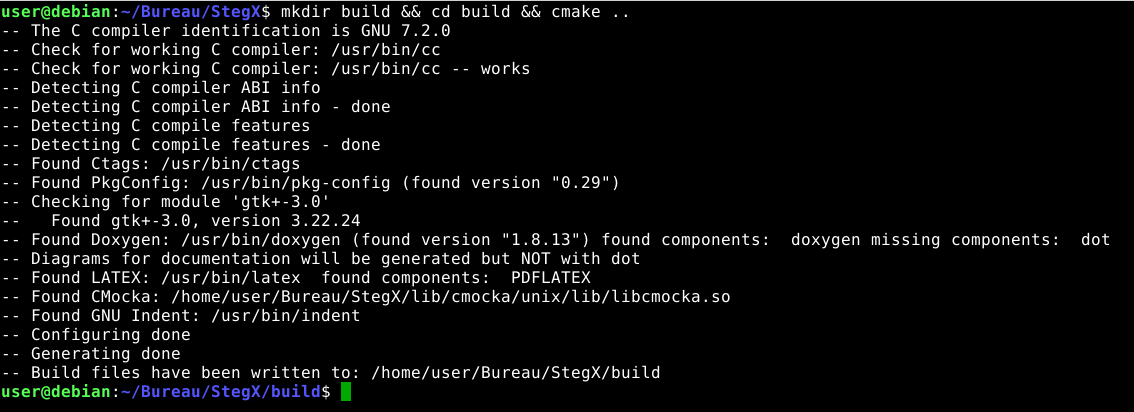
\includegraphics[scale=0.5]{pictures/build.png}
\vspace{0.5cm}

\begin{itemize}
\item make
\end{itemize}

\hspace{2cm}
\vspace{0.5cm}
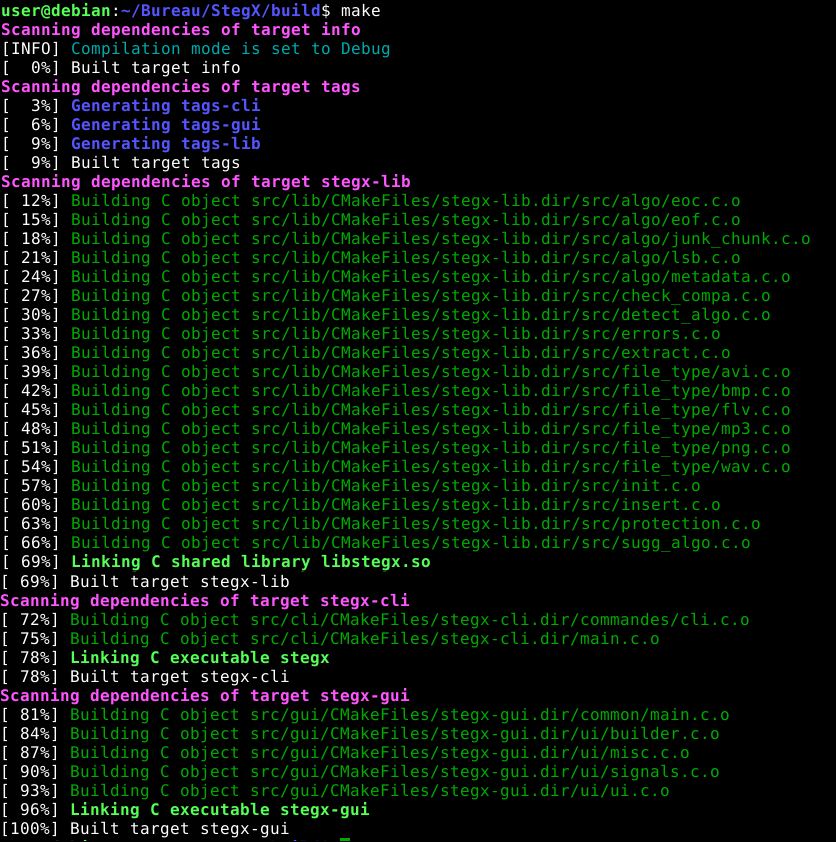
\includegraphics[scale=0.5]{pictures/make.png}


\begin{itemize}
\item sudo make install
\end{itemize}

\hspace{1cm}
\vspace{0.5cm}
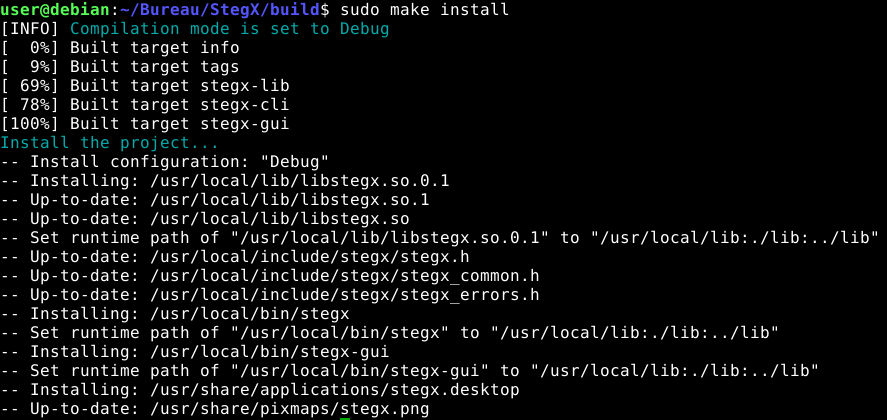
\includegraphics[scale=0.5]{pictures/install.png}

\underline{OU BIEN}

\begin{itemize}
\item Dans la section `Release`, télécharger le fichier `StegX-xxx.deb`.
\item Installer le en utilisant une interface à APT (par exemple en double cliquant
dessus), ou en utilisant la commande `sudo apt-get install ./StegX-xxx.deb`
depuis le répertoire de téléchargement.
\end{itemize}

\subsection{Désinstallation sous Linux}

Pour désinstaller StegX, taper dans sur le terminal : 
\begin{itemize}
\item sudo apt remove stegx
\end{itemize}

\subsection{Installation sous Windows}

\begin{itemize}
\item Aller sur https://www.github.com/Heisenberk/StegX/ et cliquer sur Release.
\item Télécharger l'archive et cliquer dessus à la fin du téléchargement.
\end{itemize}

\hspace{1cm}
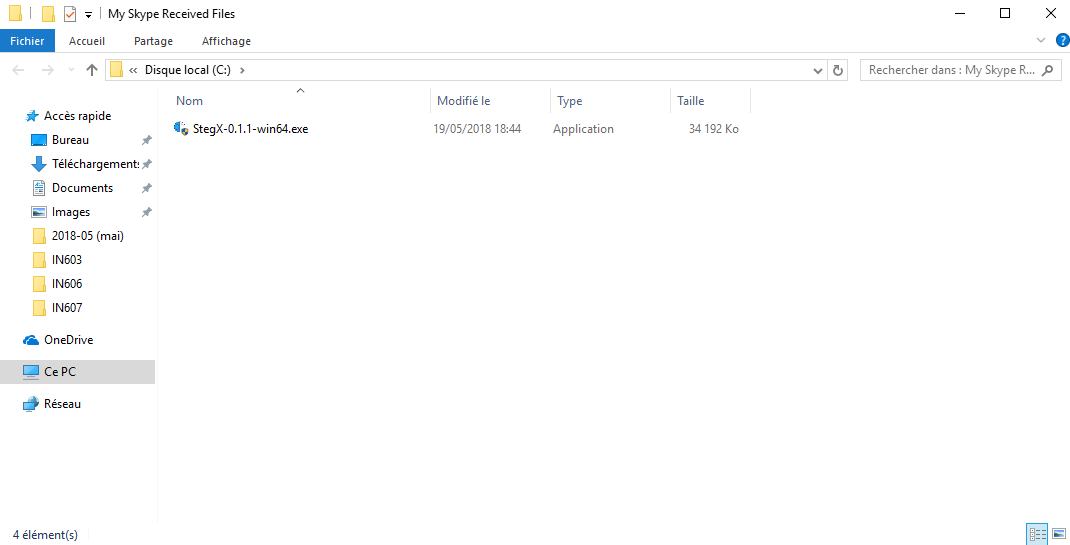
\includegraphics[scale=0.5]{pictures/ouverture.png}
\vspace{1cm}

\newpage
\begin{itemize}
\item Cliquer sur "Suivant". 
\end{itemize}

\hspace{1cm}
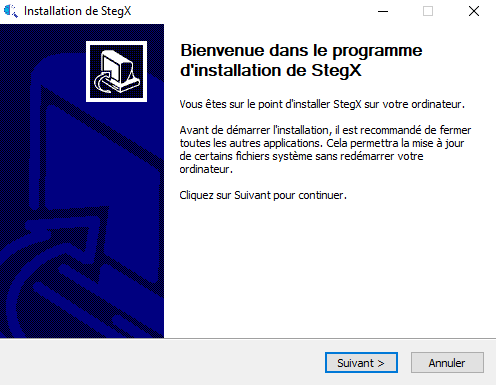
\includegraphics[scale=1]{pictures/presentation.png}
\vspace{1cm}

\begin{itemize}
\item Cliquer sur "J'accepte". 
\end{itemize}

\hspace{1cm}
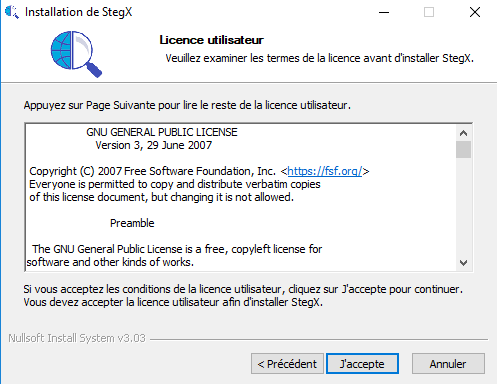
\includegraphics[scale=1]{pictures/licence.png}
\vspace{1cm}

\begin{itemize}
\item Cliquer sur "Suivant". 
\end{itemize}

\hspace{1cm}
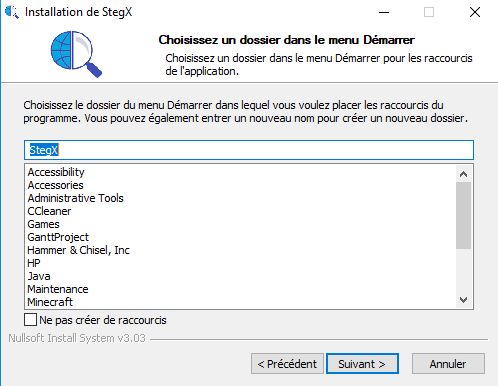
\includegraphics[scale=1]{pictures/debut.png}
\vspace{1cm}

\begin{itemize}
\item Sélectionner le premier choix. 
\item Cliquer sur "Suivant". 
\end{itemize}

\hspace{1cm}
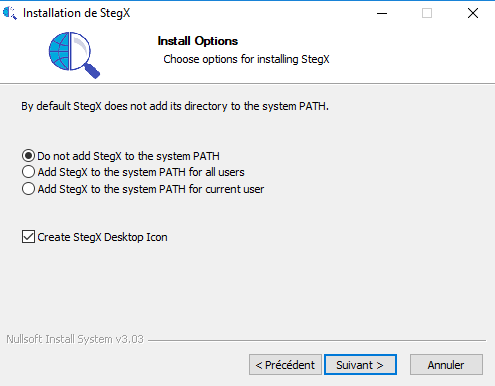
\includegraphics[scale=1]{pictures/path.png}
\vspace{1cm}

\begin{itemize}
\item Cliquer sur "Suivant". 
\end{itemize}

\hspace{1cm}
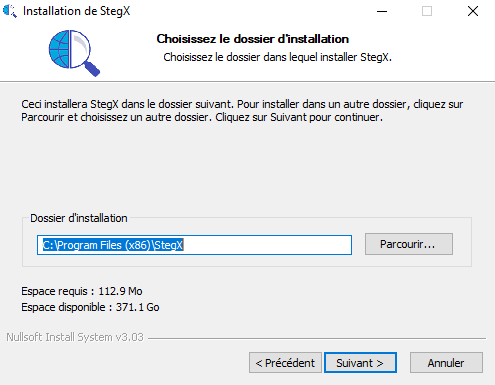
\includegraphics[scale=1]{pictures/taille.png}
\vspace{1cm}

\begin{itemize}
\item Choisir les composants de l'application à installer (interface 
en ligne de commande et/ou interface graphique). 
\end{itemize}

\hspace{1cm}
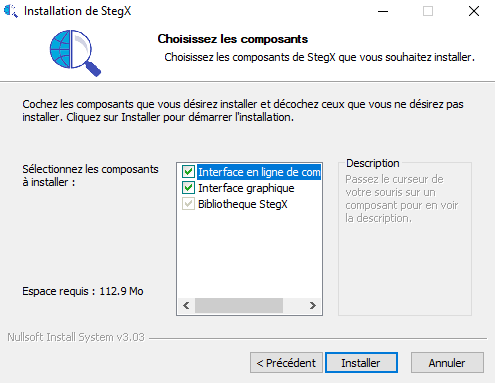
\includegraphics[scale=1]{pictures/choix.png}
\vspace{1cm}

\begin{itemize}
\item Choisir les composants de l'application à installer (interface 
en ligne de commande et/ou interface graphique). 
\item Cliquer sur "Suivant". 
\end{itemize}

\hspace{1cm}
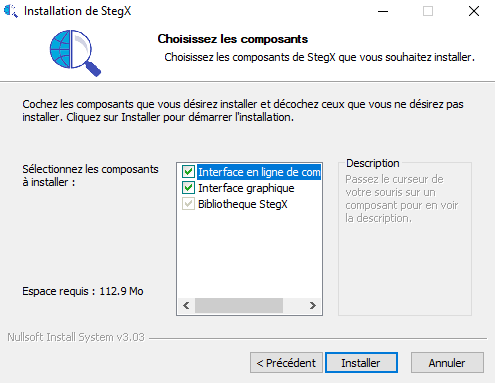
\includegraphics[scale=1]{pictures/choix.png}
\vspace{1cm}

\begin{itemize}
\item Attendre la fin de l'installation.
\item Cliquer sur "Suivant". 
\end{itemize}

\hspace{2.5cm}
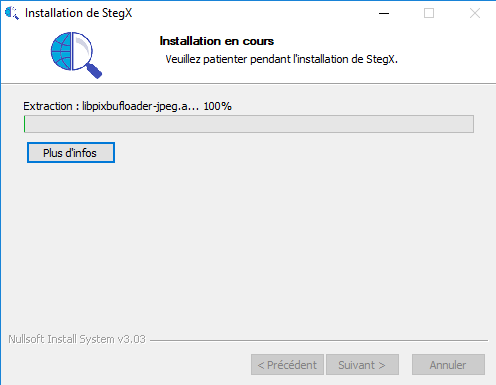
\includegraphics[scale=0.8]{pictures/installation.png}
\vspace{1cm}

\newpage
\begin{itemize}
\item Cliquer sur "Fermer". 
\end{itemize}

\hspace{1cm}
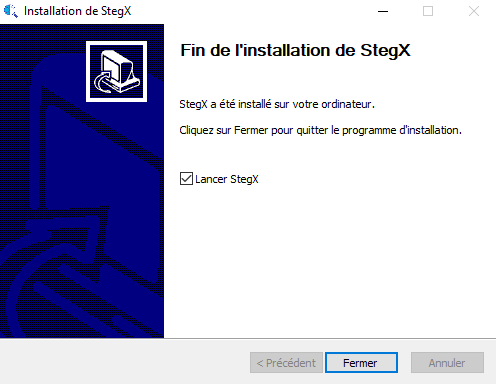
\includegraphics[scale=1]{pictures/fin.png}
\vspace{1cm}

\subsection{Désinstallation sous Windows}

\begin{itemize}
\item Accéder au panneau de configuration, cliquer sur désinstaller un programme,
sélectionner StegX et cliquer sur désinstaller.
\end{itemize}

\hspace{3cm}
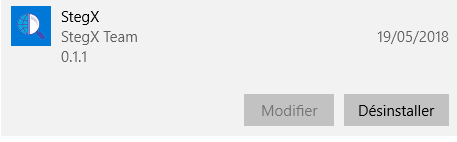
\includegraphics[scale=0.6]{pictures/desinstall.png}
\vspace{1cm}
\newpage

\section{Manuel du développeur}

\subsection{Réalisation des tests unitaires}

Pour réaliser les tests unitaires : 
\begin{itemize}
\item Aller dans le dossier "build/".
\item Taper sur le terminal "make check". Les fichiers créés seront créés 
dans le dossier "build/". 
\end{itemize}
\vspace{0.5cm}
\hspace{3cm}
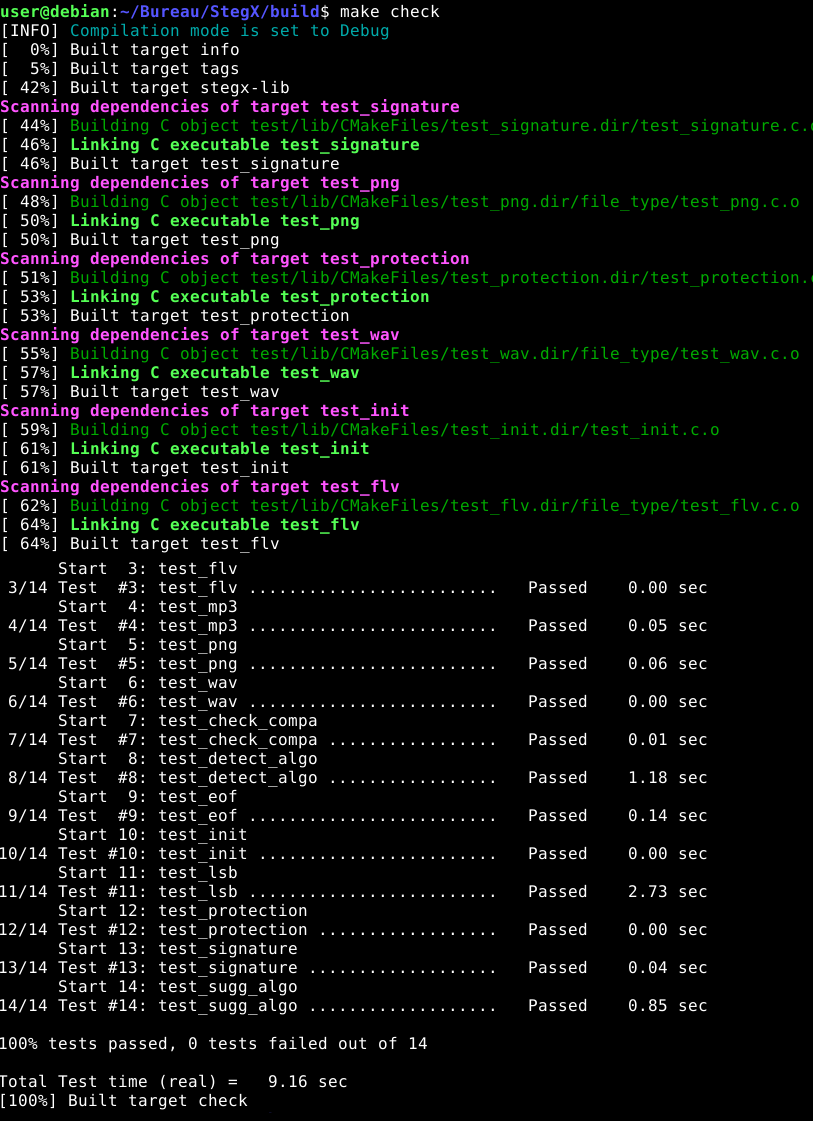
\includegraphics[scale=0.45]{pictures/check.png}
\vspace{1cm}

\subsection{Génération de la documentation}
\begin{itemize}
\item Aller dans le dossier "build/".
\item Taper sur le terminal "make doc". Les fichiers créés seront créés 
dans le dossier "build/". 
\end{itemize}
\vspace{0.5cm}
\hspace{3cm}
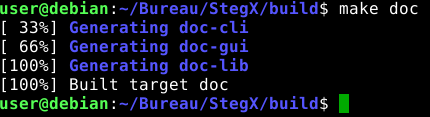
\includegraphics[scale=0.7]{pictures/doc.png}


\section{Manuel de l'utilisateur}

\subsection{Utilisation de l'interface en ligne de commande}

Pour voir la présentation de l'application en ligne de commande :
\begin{itemize}
\item Taper sur le terminal "stegx -a".
\end{itemize}

\vspace{0.5cm}
\hspace{0.5cm}
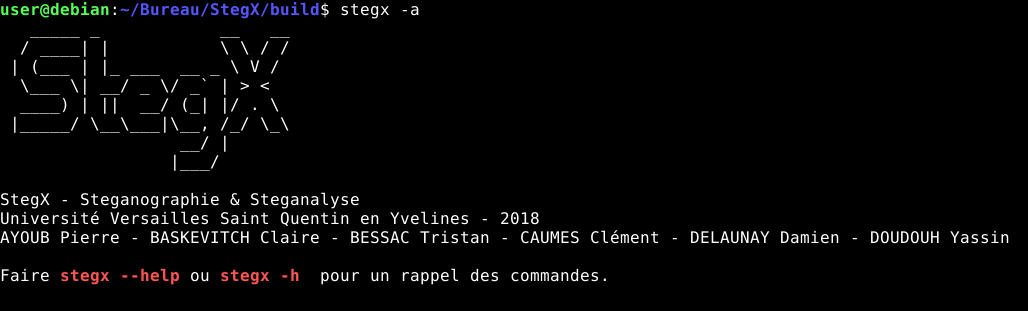
\includegraphics[scale=0.6]{pictures/present.png}
\vspace{1cm}

Pour visualiser les différentes commandes : 
\begin{itemize}
\item Taper sur le terminal "stegx -h".
\end{itemize}

\vspace{0.5cm}
\hspace{-0.5cm}
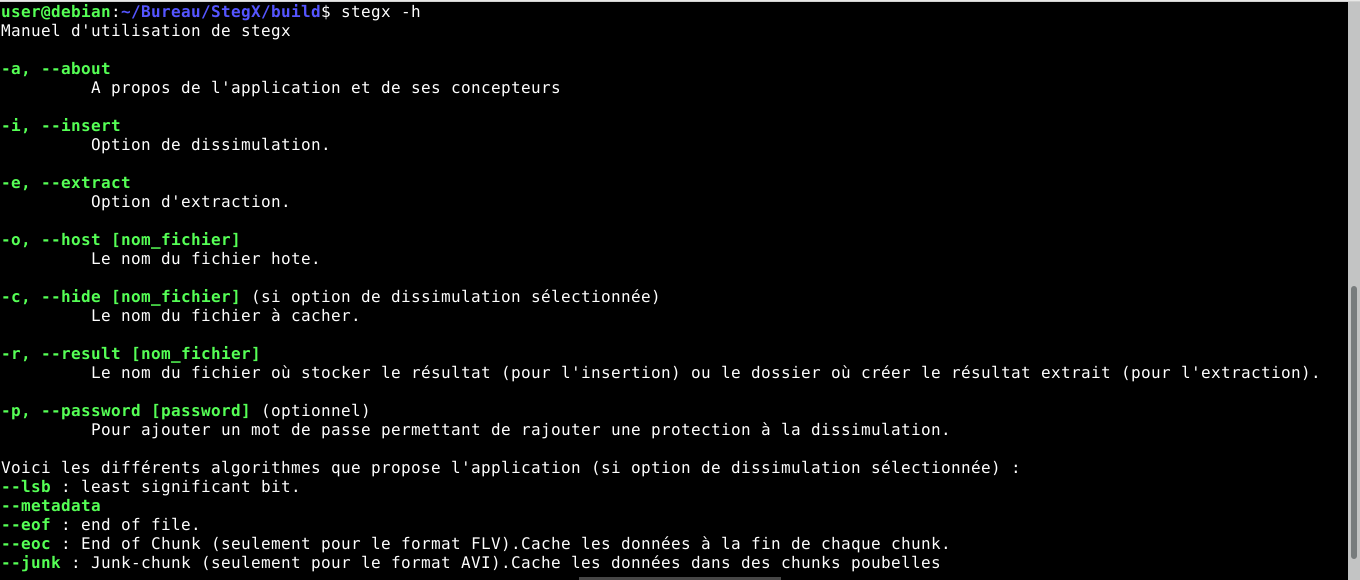
\includegraphics[scale=0.5]{pictures/help.png}
%\vspace{1cm}

\subsubsection{Insertion}

Pour réaliser une insertion, voici un exemple réalisé sur de vrais 
fichiers : 

\vspace{0.5cm}
\hspace{-2cm}
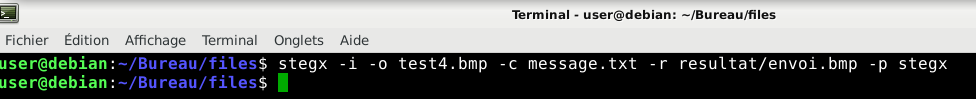
\includegraphics[scale=0.8]{pictures/insertion.png}
\vspace{1cm}

\subsubsection{Extraction}

Pour réaliser une extraction, voici un exemple réalisé sur de vrais 
fichiers :

\vspace{0.5cm}
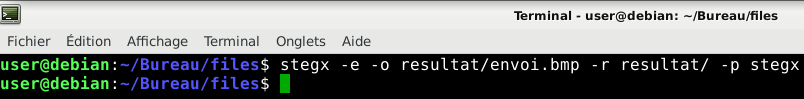
\includegraphics[scale=0.8]{pictures/extraction.png}

\subsection{Utilisation de l'interface graphique}

Pour utiliser l'application avec l'interface graphique, taper sur le 
terminal "stegx-gui" ou cliquer sur l'icône de StegX dans les raccourcis 
logiciels. 

Pour visualiser la présentation de l'application, cliquer sur "A propos". 

\vspace{0.5cm}
\hspace{2cm}
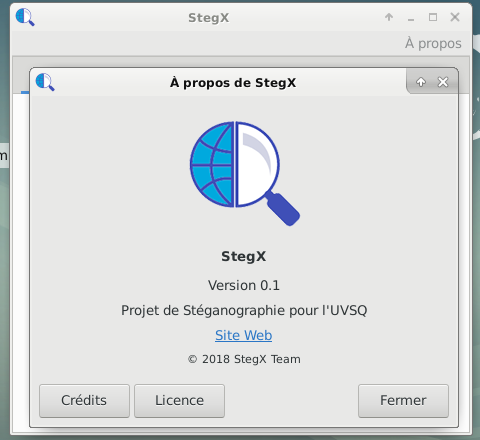
\includegraphics[scale=0.8]{pictures/a_propos.png}
\vspace{1cm}

\subsubsection{Insertion}

Pour faire une dissimulation d'un fichier à cacher dans un fichier hôte : 
\begin{itemize}
\item Cliquer sur "Dissimulation".
\item Choisir un fichier hôte. 
\item Choisir un fichier à cacher. 
\item Choisir l'emplacement du fichier à créer. 
\item Choisir un nom pour le fichier à créer. 
\item Choisir un mot de passe [facultatif]. 
\item Cliquer sur "Analyser". 
\end{itemize}

\vspace{0.5cm}
\hspace{-2cm}
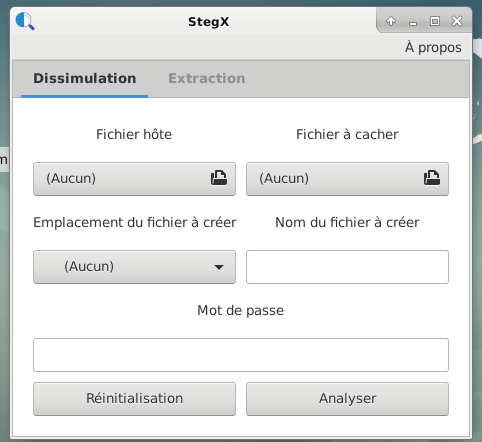
\includegraphics[scale=0.8]{pictures/ouverture2.png}
\vspace{1cm}
\hspace{0.2cm}
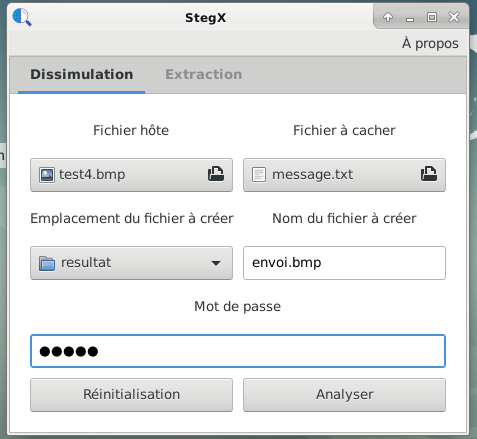
\includegraphics[scale=0.8]{pictures/insertion_1.png}

L'analyse du fichier hôte et du fichier à cacher est terminée: 
\begin{itemize}
\item Cliquer sur "Valider". 
\end{itemize}

\vspace{0.5cm}
\hspace{2cm}
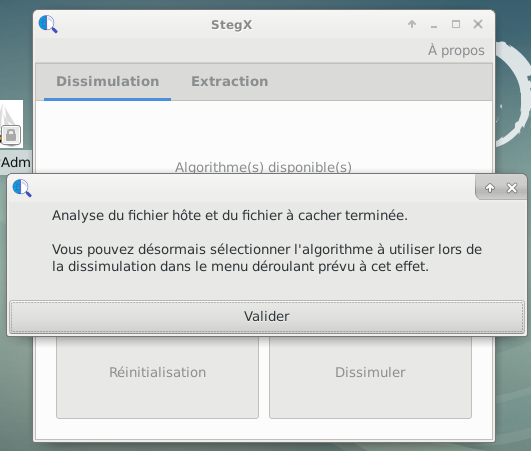
\includegraphics[scale=0.8]{pictures/insertion_2.png}
\vspace{1cm}
\newpage
Un ou plusieurs algorithmes est proposé : 
\begin{itemize}
\item Choisir l'algorithme à utiliser pour la dissimulation.
\item Cliquer sur "Dissimuler". 
\end{itemize}

\vspace{0.5cm}
\hspace{2cm}
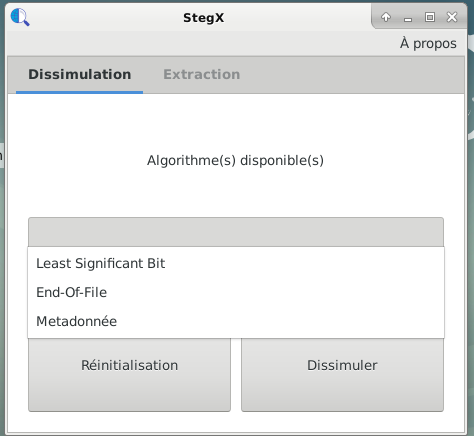
\includegraphics[scale=0.8]{pictures/insertion_3.png}


\subsubsection{Extraction}

Pour réaliser une extraction d'un fichier caché dans un fichier à analyser : 
\begin{itemize}
\item Cliquer sur "Extraction".
\item Choisir un fichier hôte (fichier à analyser). 
\item Choisir l'emplacement du fichier extrait. 
\item Choisir un mot de passe [facultatif]. 
\item Cliquer sur "Extraire". 
\end{itemize}

\vspace{1cm}
\hspace{-2cm}
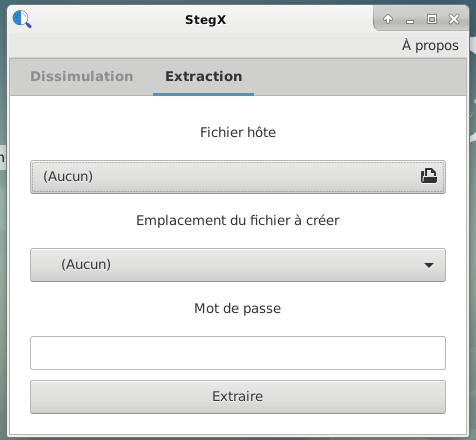
\includegraphics[scale=0.8]{pictures/extraction_1.png}
\vspace{1cm}
\hspace{0.2cm}
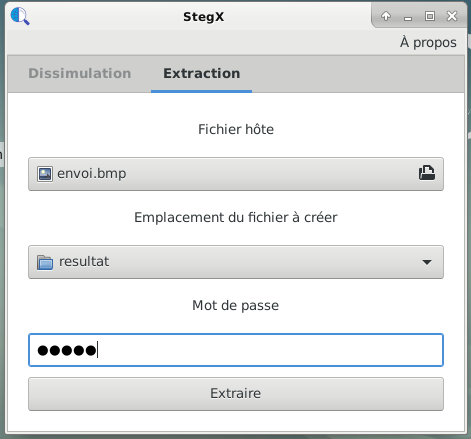
\includegraphics[scale=0.8]{pictures/extraction_2.png}

Lorsque l'extraction est terminée, une fenêtre s'ouvre : 

\vspace{0.5cm}
\hspace{2.5cm}
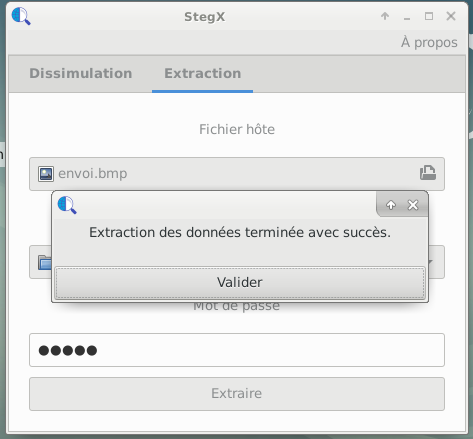
\includegraphics[scale=0.8]{pictures/extraction_3.png}
\vspace{1cm}

\end{document}
